

% The landing system is structured as a system of \gls{ROS} modules, as shown in Figure \ref{fig:landing_system_architecture}. The first is the \texttt{roscore} module which is necessary within the \gls{ROS} framework and which functions as a base server to facilitate communication among the other \gls{ROS} modules. The data flow is as follows:

% \begin{enumerate}
%     \item The drone-mounted camera provides a raw image of the landing pad's fiducial marker.
%     \item The \texttt{usb\_cam} module provides the raw image from the camera to the rest of the \gls{ROS} modules as a topic.
%     \item The \texttt{whycon\_ros} module analyzes the camera frames and attempts to detect and identify WhyCon markers within the image. If it detects a WhyCon marker, it provides the location and rotation of the marker relative to the camera.
%     \item The \texttt{landing\_controller} module monitors the position of the fiducial marker over time, simultaneously determining the relative velocity. It generates an approach trajectory and communicates this in the MAVlink protocol to the ArduPilot software via the \texttt{mavros} module.
%     \item The \texttt{abort\_controller} module continuously monitors the \gls{IMU} conditions of the drone and the visibility of the fiducial marker in order to determine whether an in-progress landing should be aborted.
%     \item The \texttt{mavros} module provides an interface to allow the \gls{ROS} modules to communicate to the ArduPilot software using the MAVlink communication protocol.
% \end{enumerate}

% \begin{figure}[H]
%     \centering
%     %\makebox[\textwidth][c]{
%     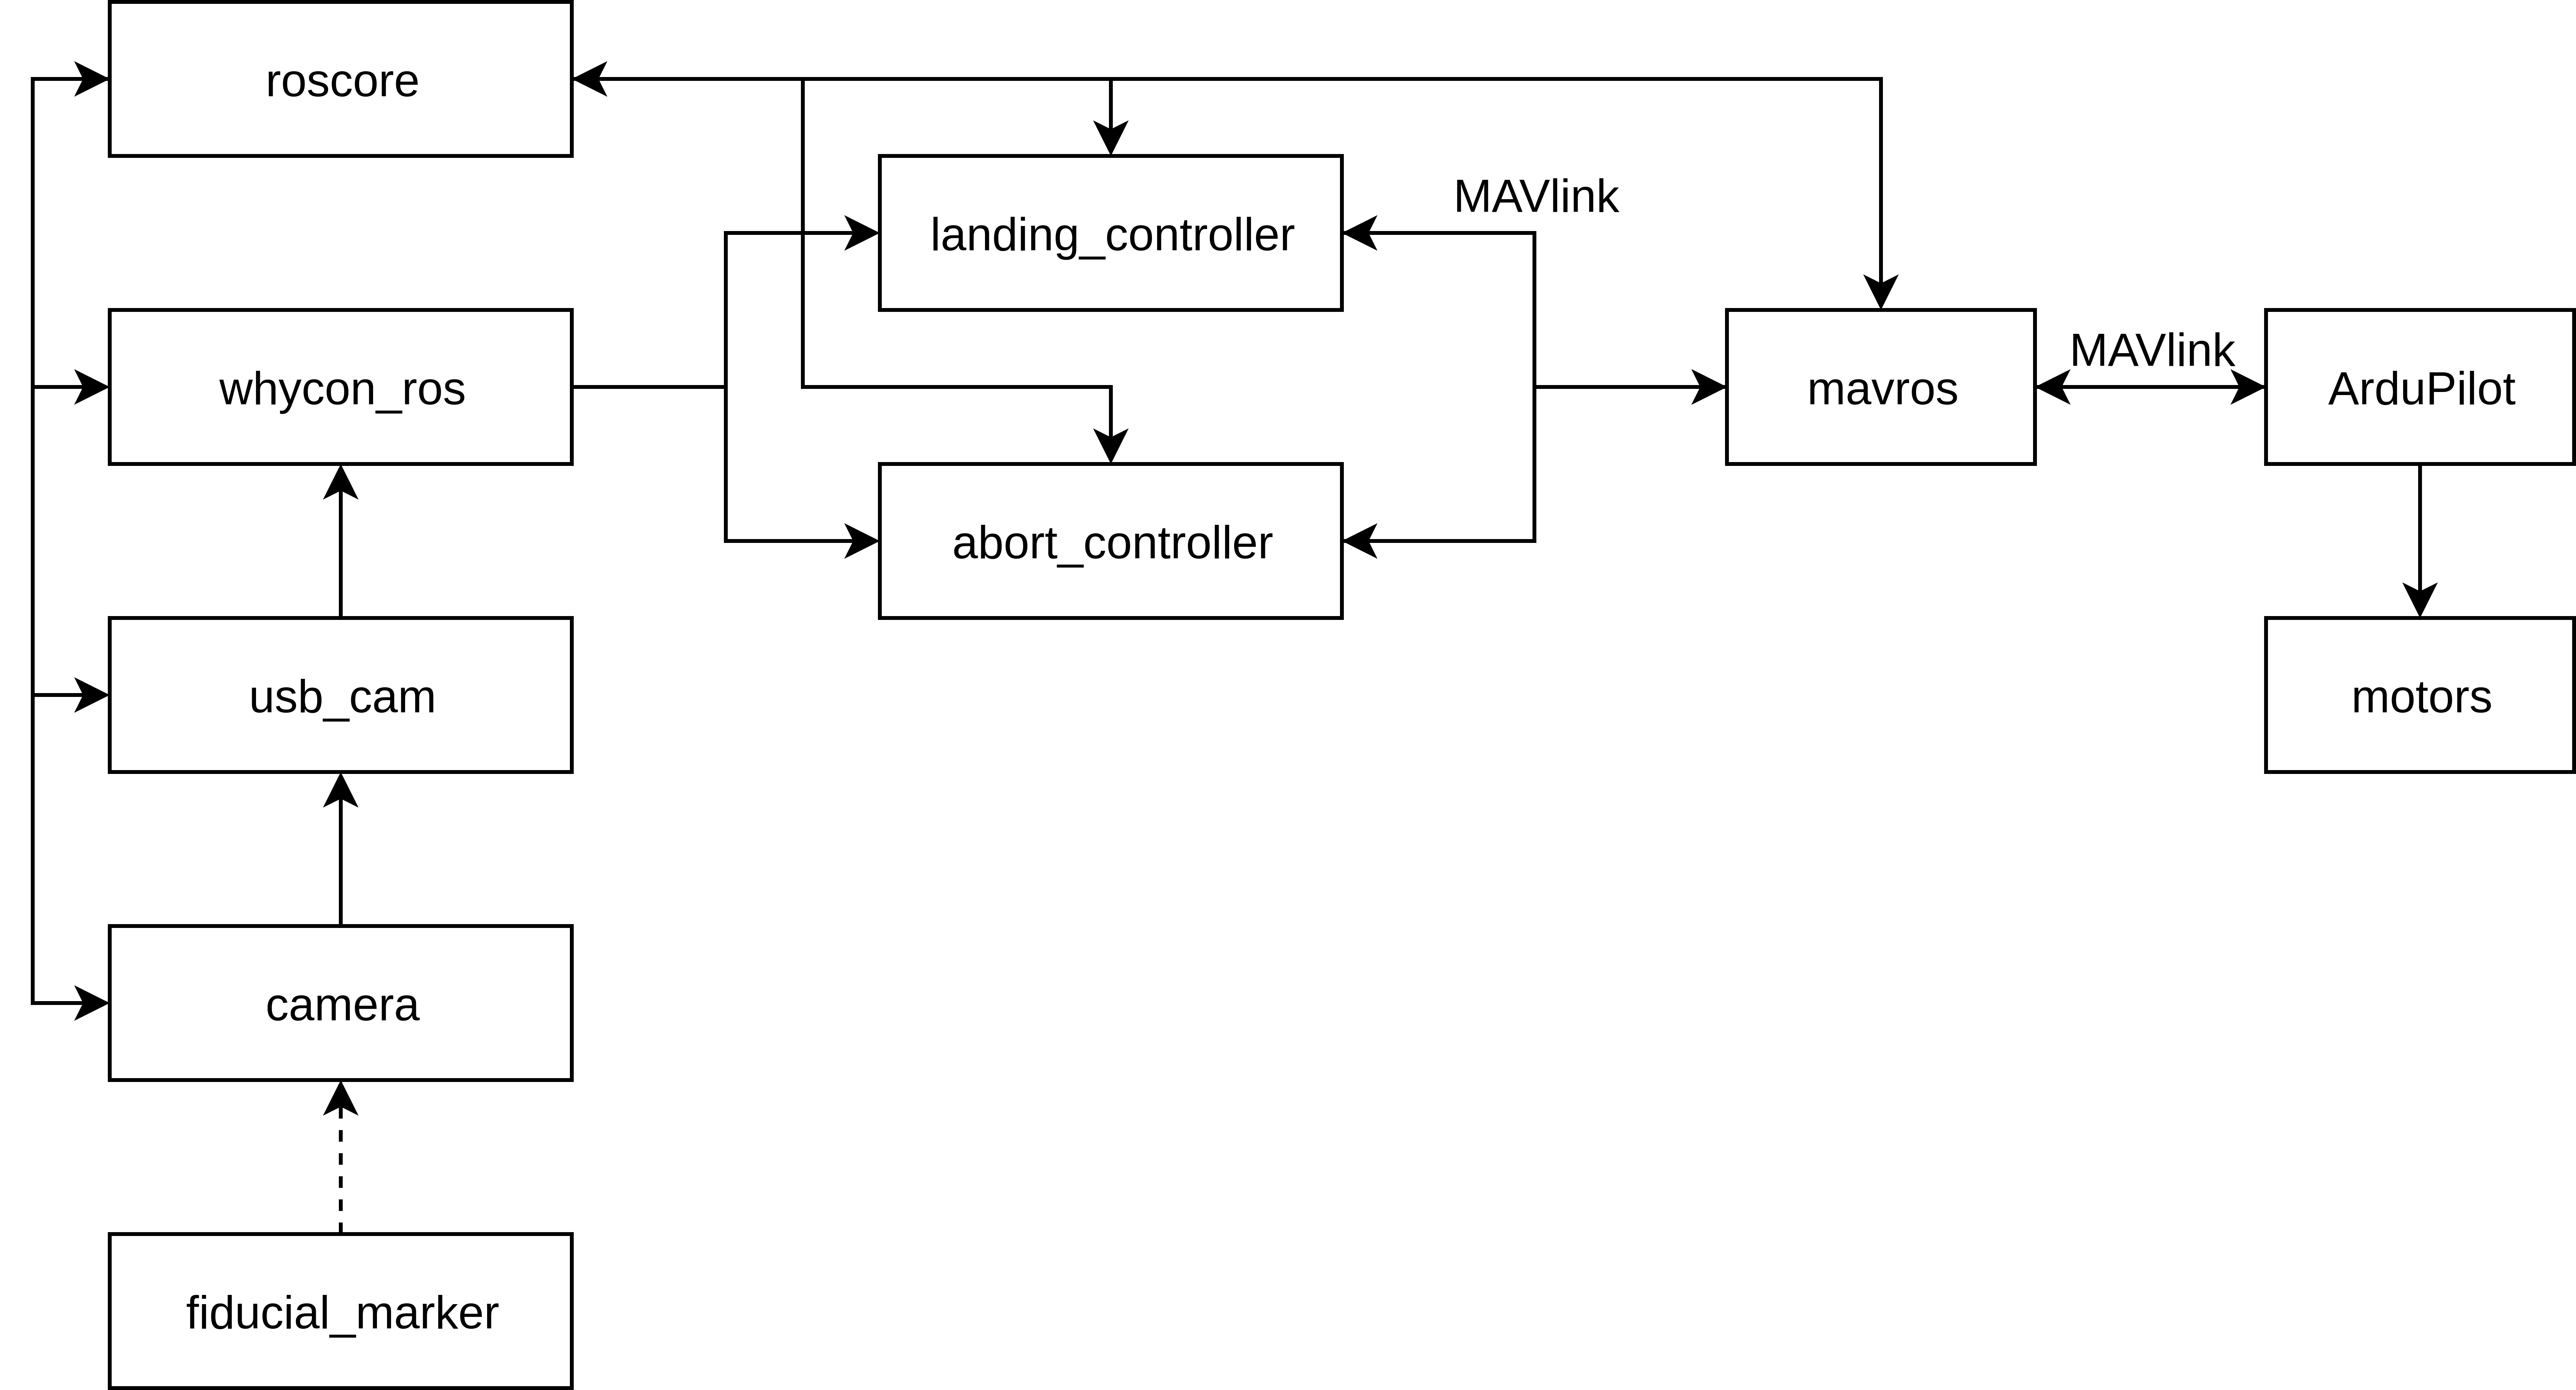
\includegraphics[width=\textwidth]{images/system_architecture.png}
%     %}
%     \caption{High level landing system architecture.}
%     \label{fig:landing_system_architecture}
% \end{figure}